\documentclass[]{standalone}
\usepackage{amsmath}
\usepackage{amssymb}
% No page numbers and no paragraph indentation                                  
\pagestyle{empty}                                                               
\setlength{\parindent}{0bp}%
\usepackage{graphicx}
\usepackage{tikz}
\usepackage{xcolor}
\usetikzlibrary{calc,fadings,decorations.pathreplacing,shapes,shapes.multipart,arrows,shapes.misc,intersections,positioning}

\begin{document}

\tikzset{
    partial ellipse/.style args={#1:#2:#3}{
        insert path={+ (#1:#3) arc (#1:#2:#3)}
    }
}

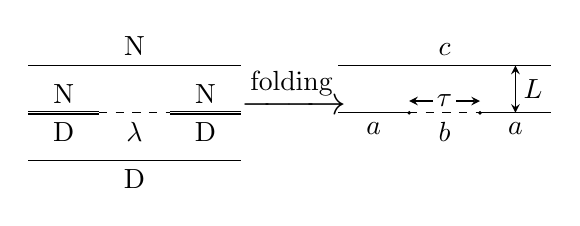
\begin{tikzpicture}[scale = 0.75]
\draw (0,0.2) -- ++(3.6,0);
\draw (0,1.8) -- ++(3.6,0);
\draw (0,1.02) --++( 1.2, 0);
\draw (0,0.98) --++( 1.2, 0);
\draw[dashed] (1.2,1) --++( 1.2, 0);
\draw (2.4,1.02) --++( 1.2, 0);
\draw (2.4,0.98) --++( 1.2, 0);
\node[above] () at (1.8,1.8) {N};
\node[below] () at (1.8,0.2) {D};
\node[above] () at (0.6,1) {N};
\node[below] () at (0.6,1) {D};
\node[above] () at (3,1) {N};
\node[below] () at (3,1) {D};
\node[below] () at (1.8,1) {$\lambda$};
\node[above] () at (4.5,0.8) {\Large $\xrightarrow{\rm folding}$};

\begin{scope}[shift={(5.25,0.)}]
\draw (0,1) -- (1.2,1);
\draw (2.4,1) -- ++(1.2,0);
\draw[dashed] (1.2,1) -- (2.4,1);
\draw[fill] (1.2,1) circle (0.02);
\draw[fill] (2.4,1) circle (0.02);
\draw (0,1.8) -- (3.6,1.8);
\draw[stealth-stealth] (3,1.8)--(3, 1);
\node () at (3.3,1.4) {$L$};
\node[below] () at (0.6,1) {$a$};
\node () at (1.8,1.2) {$\tau$};
\draw[-stealth] (1.6, 1.2) -- (1.2, 1.2);
\draw[-stealth] (2, 1.2) -- ++(0.4, 0);
\node[below] () at (1.8,1) {$b$};
\node[below] () at (3,1) {$a$};
\node[above] () at (1.8,1.8) {$c$};
\end{scope}
\end{tikzpicture}


\end{document}